% --------------------------------------------------------------------------
% Template for IWAENC 2022 papers; to be used with:
%          spconfa4.sty  - ICASSP/ICIP LaTeX style file, and
%          IEEEbib.bst - IEEE bibliography style file.
%
% (Last modified by H. Loellmann, LMS, FAU Erlangen-Nuremberg, Jan. 2020)
%
% --------------------------------------------------------------------------

\documentclass{article}
\usepackage[preprint]{spconfa4}
\usepackage{amsmath,graphicx}
\usepackage[dvipsnames]{xcolor}
\usepackage{tikz}
\usetikzlibrary{arrows,snakes,backgrounds,matrix,patterns,positioning,fadings}
\usepackage{standalone}
\usepackage{subfig}
\usepackage{upgreek}
\usepackage{nicefrac}
\usepackage{dsfont}
\usepackage{bm}
\usepackage{cancel}
\usepackage{amsbsy}
\usepackage{algorithm}
\usepackage{algpseudocode}
\usepackage{lipsum}
\usepackage{harpoon}
\usepackage{comment}
\newenvironment{note}
 {\par\textcolor{Blue}{\bfseries Note:} \color{Blue}\ignorespaces}
 {\par}
\newenvironment{attention}
 {\par\textcolor{red}{\bfseries Attention:} \color{red}\ignorespaces}
 {\par}
\usepackage{hyperref}
\hypersetup{
	colorlinks,
	linkcolor={blue!80!black},
	citecolor={blue!80!black},
	urlcolor={blue!80!black}
}

\newcommand{\mtxb}[1]{\bm{\mathrm{#1}}}
\newcommand{\T}{{\mathrm{T}}}
\newcommand{\herm}{{\mathrm{H}}}
\newcommand{\ev}[1]{\mathrm{E} \left\lbrace #1 \right\rbrace}

% IMPORTANT: Add copyright notice by uncommenting the appropriate line
%----------------------------------------------------------
% For papers in which all authors are employed by the US government,
% \copyrightnotice{U.S. Government work not protected by U.S. copyright}

% For papers in which all authors are employed by a Crown government (UK, Canada, and Australia)
% \copyrightnotice{978-1-6654-6867-1/22/\$31.00~\copyright2022 Crown}
                   
% For papers in which all authors are employed by the European Union,
% \copyrightnotice{978-1-6654-6867-1/22/\$31.00~\copyright2022 European Union}
                   
% For all other papers the copyright notice is
\copyrightnotice{978-1-6654-6867-1/22/\$31.00~\copyright2022 IEEE}
                   
% Title.
% ------
\title{CROSS-RELATION BASED BLIND SYSTEM IDENTIFICATION USING ADMM}
%
% Single address.
% ---------------
\name{Matthias Blochberger\sthanks{THANK EU!}, Filip Elvander\sthanks{THANK FWO?}, Randall Ali, Toon van Waterschoot}
\address{KU Leuven\\ESAT - Department of Electrical Engineering\\STADIUS\\3001 Leuven}
%
% For example:
% ------------
%\address{School\\
%	Department\\
%	Address}
%
% Two addresses (uncomment and modify for two-address case).
% ----------------------------------------------------------
%\twoauthors
%  {A. Author-one, B. Author-two\sthanks{Thanks to XYZ agency for funding.}}
%	{School A-B\\
%	Department A-B\\
%	Address A-B}
%  {C. Author-three, D. Author-four\sthanks{The fourth author performed the work
%	while at ...}}
%	{School C-D\\
%	Department C-D\\
%	Address C-D}
%
\begin{document}
%\ninept
%
\maketitle
%
\begin{abstract}
The abstract should appear at the top of the left-hand column of text, about 0.5 inch (12 mm) below the title area and no more than 3.125 inches (80 mm) in length.
Leave a 0.5 inch (12 mm) space between the end of the abstract and the beginning of the main text.
The abstract should contain about 100 to 150 words, and should be identical to the abstract text submitted electronically.
All manuscripts must be in English.
\end{abstract}
%
\begin{keywords}
One, two, three, four, five
\end{keywords}
%
\section{Introduction}
\label{sec:intro}

These guidelines include complete descriptions of the fonts, spacing, and related information for producing your proceedings manuscripts.
If you have any questions regarding the paper submission, please contact the conference organizers via email: \texttt{submission@iwaenc2022.org}\,.

\section{Problem statement}
\label{sec:problem_statement}


\section{Distributed BSI}
\label{sec:admm_bsi}

\subsection{ADMM?}
\label{ssec:admm}

\section{Numerical Evaluation}
\label{sec:num_eval}



\section{Conclusion}
\label{sec:conclusion}


% \begin{figure}[tb]
	
% 	\begin{minipage}[b]{1.0\linewidth}
% 		\centering
% 		\centerline{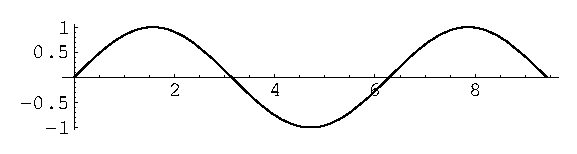
\includegraphics[width=8.5cm]{image1}}
% 		%  \vspace{2.0cm}
% 		\centerline{(a) Result 1}\medskip
% 	\end{minipage}
% 	%
% 	\begin{minipage}[b]{.48\linewidth}
% 		\centering
% 		\centerline{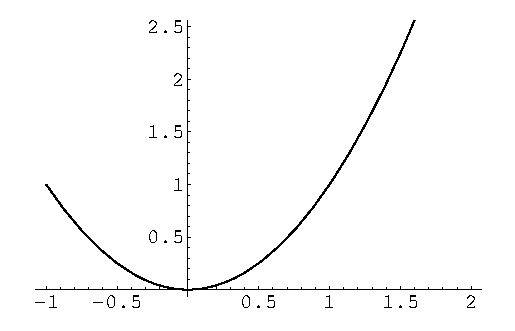
\includegraphics[width=4.0cm]{image3}}
% 		%  \vspace{1.5cm}
% 		\centerline{(b) Results 2}\medskip
% 	\end{minipage}
% 	\hfill
% 	\begin{minipage}[b]{0.48\linewidth}
% 		\centering
% 		\centerline{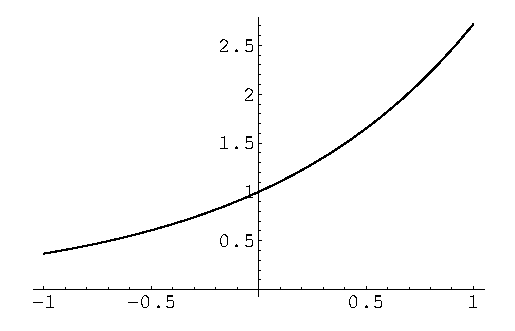
\includegraphics[width=4.0cm]{image4}}
% 		%  \vspace{1.5cm}
% 		\centerline{(c) Result 3}\medskip
% 	\end{minipage}
% 	%
% 	\caption{Example of placing a figure with results.}
% 	\label{fig:example}
% 	%
% \end{figure}

% References should be produced using the bibtex program from suitable
% BiBTeX files (here: strings, refs, manuals). The IEEEbib.bst bibliography
% style file from IEEE produces unsorted bibliography list.
% -------------------------------------------------------------------------
% \bibliographystyle{IEEEbib}
% \bibliography{refs}

\end{document}